% !TEX program = xelatex
% 编译: xelatex 论文.tex  (两遍)
\documentclass[11pt,a4paper]{ctexart}
\usepackage[a4paper,top=2.4cm,bottom=2.4cm,left=2.6cm,right=2.6cm]{geometry}
\usepackage{amsmath,amssymb}
\usepackage{booktabs}
\usepackage{graphicx}
\usepackage{float}
\usepackage{caption}
\usepackage{array}
\usepackage{multirow}
\usepackage[colorlinks=true,linkcolor=blue,citecolor=blue]{hyperref}
\graphicspath{{figs/}}
\captionsetup{font=small,labelfont=bf}
\setlength{\parskip}{2pt}
\renewcommand{\arraystretch}{1.25}
\newcommand{\E}{\mathbb{E}}

\begin{document}

\begin{center}
  {\LARGE\bfseries NIPT 的时点选择与胎儿的异常判定\par}
  \vspace{4pt}
  {\large 基于纵向混合效应模型与风险--可靠性双目标决策\par}
  \vspace{10pt}
  {\large 数学建模竞赛论文\par}
  \vspace{2pt}
  {\normalsize 2026年9月}
\end{center}

\vspace{8pt}
\begin{abstract}
\noindent 针对无创产前检测（NIPT）时点选择与胎儿染色体异常判定问题，本文基于某高 BMI 地区孕妇的男胎纵向重复测量数据（1082 条、267 名孕妇）与女胎数据（605 条、147 名孕妇），按"机理关联 $\to$ 个体时点决策 $\to$ 多因素稳健化 $\to$ 判别分类"的递进路线建立系列模型。\textbf{问题一}：联合行级/个体级相关分析、面板固定效应与线性混合效应模型（随机截距+随机斜率）刻画 Y 染色体浓度与孕周、BMI 的关系：组内孕周斜率 $0.0035$/周（$p<10^{-4}$），BMI 每增 1 个单位个体浓度水平约降 $0.12$ 个百分点（$p=0.023$）；个体间差异占总变异的 $ICC=0.81$、条件 $R^2=0.84$，说明统一时点必然牺牲部分孕妇的准确性。\textbf{问题二}：以"浓度达 $4\%$ 的最早孕周 $\tau$"为桥梁，用 BLUP 法与插值法双路估计个体达标时间（Spearman $\rho=0.73$），建立平滑风险函数 $w(t)=e^{(\ln 4/9)(t-11)}$（11/20/29 周处风险 $1:4:16$）下的期望风险模型，并采用"风险最小 + 风险平带内单次达标率最高"双判据；组间检验表明 BMI=36 是唯一显著分界（Mann--Whitney $p<10^{-6}$），推荐 \textbf{BMI$<36$ 组 11 周首检、BMI$\ge36$ 组 14.5 周首检}，较经验"五档统一 12 周"方案期望风险降低约 $4\%$、人均抽血 1.86$\to$1.77 次，并经 400--600 次参数自助给出时点稳健区间与灵敏度结果。\textbf{问题三}：嵌套似然比检验表明年龄/身高/体重在孕周+BMI 之上的增量信息有限（$R^2\le0.12$），维持 BMI 分档并给出达标比例 $0.7\sim0.95$ 约束下的风险--达标率权衡表；量化测量噪声 $\sigma_m=0.009$（约合 $\tau$ 的 2.6 周不确定度）与到检执行偏差（$\pm0.5$ 周）的影响，时点结论稳健。\textbf{问题四}：以女胎 AB 列为金标准，构建"QC 门控（通过率 63.4\%）$+$ 逻辑回归/随机森林（按孕妇分组交叉验证，行级 OOF AUC$=0.803$；T13/T18/T21 分别为 0.758/0.832/0.576）$+$ 等渗概率校准（Brier 0.158$\to$0.074）$+$ 多胎次证据整合（$\ge2$ 次独立阳性才报高风险，特异性/PPV 达 100\%）"的分层判定流水线；并核查出 AB 标签与单次 Z 值规则脱节、孕妇多次检测标签不一致率达 29.3\% 等数据特征，给出对应的保守复核建议。
\end{abstract}

\vspace{2pt}
\noindent\textbf{关键词}：NIPT；线性混合效应模型；个体最早达标时间；期望风险决策；逻辑回归与概率校准；非整倍体判定

\tableofcontents
\newpage

%============================================================
\section{问题重述}
NIPT 通过检测孕妇外周血中胎儿游离 DNA 评估胎儿染色体非整倍体异常（唐氏 T21、爱德华 T18、帕陶 T13）。临床经验中，男胎以 Y 染色体浓度是否达到 $4\%$ 判定检测结果是否基本准确；该浓度与孕妇孕周、身体质量指数（BMI）等密切相关，且孕妇个体差异（年龄、BMI、孕情等）显著。若统一检测时点过早，浓度不足导致测序失败与复查；过晚则使不健康胎儿的发现孕周后移、治疗窗口缩短：12 周以内发现风险较低，13--27 周风险高，28 周以后风险极高。基于某高 BMI 地区孕妇的 NIPT 纵向数据（男胎 1082 条记录 / 267 名孕妇；女胎 605 条记录 / 147 名孕妇），需要解决：

\begin{enumerate}
\item 分析胎儿 Y 染色体浓度与孕妇孕周、BMI 等指标的相关特性，给出关系模型并检验其显著性；
\item 临床证明 BMI 是影响 Y 浓度最早达标时间的主要因素：对男胎孕妇按 BMI 合理分组，给出各组的 BMI 区间与最佳 NIPT 时点，使孕妇潜在风险最小，并分析检测误差的影响；
\item 男胎达标时间受身高、体重、年龄等多种因素影响：综合考虑这些因素、检测误差与达标比例（浓度 $\ge4\%$ 的比例），按 BMI 给出合理分组及每组最佳时点，使风险最小并分析误差影响；
\item 对女胎，以 AB 列（13/18/21 号染色体非整倍体）为判定结果，综合考虑 X 染色体及相关染色体的 Z 值、GC 含量、读段数及相关比例、BMI 等因素，给出女胎异常的判定方法。
\end{enumerate}

\section{问题分析}
\textbf{整体数据流}：四个问题共用同一孕妇纵向数据，但层次递进。问题一建立"浓度--时间--体质"的定量关系（机理关联层）；问题二在其上推导个体最早达标时间 $\tau$，将"时点选择"转化为"达标时间分布下的期望风险最小化"（决策层）；问题三在决策层加入多因素协变量、达标比例约束与误差传播（稳健精细化）；问题四面向女胎独立成分类判别问题（判别层）。

\begin{description}
\item[问题一（本质：重复测量面板回归）] 难点在于个体差异与观测时点的混杂：高 BMI 孕妇往往更晚首次受检，行级简单相关会低估甚至掩盖孕周效应。处理分三步：先以面板固定效应（组内去均值）分离时间趋势；再以线性混合效应模型（随机截距+随机斜率）同时刻画总体趋势、个体水平差异与个体增长速率差异；最后做嵌套似然比检验与方差分解（ICC），定量回答"统一时点是否合理"。
\item[问题二（本质：不确定性下的决策优化）] 个体最早达标时间 $\tau$ 未知且有分布。若统一首检时点 $t<\tau$，检测不可靠、需复查并顺延确诊；若 $t$ 过晚则推迟异常确诊。定义"发现孕周" $d(t,\tau)$ 与风险权重 $w(d)$，组最优时点 $t_g^{*}=\arg\min_t \E[w(d)]$；分组的合理性以组间 $\tau$ 差异检验（Kruskal--Wallis、Mann--Whitney）与数据驱动分界点联合搜索共同判定。
\item[问题三（本质：多因素增量检验 + 多目标权衡）] 先检验身高/体重/年龄相对 BMI 的增量信息（似然比、AIC/BIC、未截断子样本回归 $R^2$）；再在 $P(\tau\le t)\ge p_0$ 的达标比例约束下重解时点，给出权衡表；最后用参数自助传播三类误差（浓度测量噪声、复查延迟、到检执行偏差）。
\item[问题四（本质：类不平衡判别）] 阳性行仅占 11.1\%。数据核查发现 AB 标签与单次 Z 值规则显著脱节（T18 阳性行 $z_{18}>3$ 占比 $0\%$；29.3\% 孕妇多次检测标签不一致），故采用"质量门控 $+$ 多特征联合判别 $+$ 概率校准 $+$ 多胎次证据整合"的保守流水线，评估协议按孕妇分组交叉验证、OOF 概率与置换检验，杜绝重复样本泄漏与乐观偏差。
\end{description}

\section{模型假设与符号说明}
\subsection{基本假设}
\begin{enumerate}
\item Y 染色体浓度在观测窗（11--28 周）内随孕周近似线性增长：组内去均值回归斜率极显著（$p\approx10^{-103}$）且各 BMI 段斜率一致；
\item 给定孕妇个体水平，其不同次检测相互独立；同周重复检测的波动可视为纯测量噪声 $\sigma_m$ 的估计来源；
\item 浓度 $\ge4\%$ 时 NIPT 结果基本准确，否则本次检测不可靠，复查后约延迟 $\Delta$ 周才能可靠检出（$\Delta$ 默认 1.5 周，敏感性 0.5--3 周）；
\item 异常胎儿发现风险仅取决于发现孕周，风险随孕周按"低/高/极高"非线性放大，以平滑函数 $w(t)=e^{k(t-11)}$、$k=\ln4/9$ 逼近（在 11、20、29 周处分别取 1、4、16）；
\item 各 BMI 组胎儿异常基础发生率 $q$ 近似相同。因 $q$ 是公共乘性常数，$\arg\min_t q\E[w(d)]$ 与 $q$ 无关，选时点无需估计 $q$；
\item 身高、体重、年龄在孕期内视为时不变协变量（数据中同孕妇多次记录一致）。
\end{enumerate}

\subsection{主要符号}
\begin{table}[H]
\centering\small
\caption{主要符号说明}
\begin{tabular}{llll}
\toprule
符号 & 含义 & 符号 & 含义\\
\midrule
$y_{it}$ & 孕妇 $i$ 在孕周 $t$ 的 Y 浓度 & $t_g$ & $g$ 组统一首检时点\\
$\mathrm{BMI}_i$ & 孕妇 BMI（另：$a,h,m$ 为年龄/身高/体重） & $d_i(t)$ & 时点 $t$ 下孕妇 $i$ 的发现孕周\\
$\tau_i$ & 个体最早达标时间：$y_i(\tau_i)=4\%$ & $w(\cdot)$ & 风险权重函数\\
$u_{0i},u_{1i}$ & 个体随机截距/随机斜率（BLUP） & $R_g(t)$ & $g$ 组期望风险 $\E[w(d)]$\\
$\Delta$ & 复查延迟（周） & $\sigma_m$ & 浓度测量噪声标准差\\
$z_{13},z_{18},z_{21},z_X$ & 各染色体 Z 值 & $c_X$ & X 染色体浓度\\
\bottomrule
\end{tabular}
\end{table}

\section{数据预处理与探索性分析}
\textbf{清洗与解析}：孕周以 `11w+6`、`16w`、`16W+1` 等格式给出，统一解析为小数周（部分记录不带天数，按 $+0$ 处理）；按 $\mathrm{BMI}=m/h^2$ 反算校验题给 BMI 列，最大偏差 $<0.1\%$，仅剔除 1 行 BMI 缺失；女胎表含两列无名占位列（对应男胎 Y 染色体 Z 值与浓度），按附录 1 对齐后丢弃。男胎存在 41 组"同一孕妇同孕周重复检测"，据此估计测量噪声 $\sigma_m=0.00903$（浓度单位），约为 $4\%$ 阈值的 $22.6\%$，按斜率折算约合 $\tau$ 的 $2.6$ 周不确定度。

\textbf{描述统计}：男胎浓度均值 7.7\%、中位 7.5\%、范围 1.0--23.4\%，达标行占 86.6\%；BMI 20.7--46.9（中位 31.8，符合高 BMI 人群）；孕周 11.0--27.7；女胎异常标注行 67/605（11.1\%），孕妇级阳性 44/147（29.9\%）。

\textbf{三个关键观察}（引导后续建模）：
\begin{enumerate}
\item \emph{行级弱相关、组内强趋势}：行级浓度--孕周 Pearson $r=0.124$（$p=4\times10^{-5}$），而组内去均值斜率 $+0.0032\sim0.0035$/周（$p\approx10^{-103}$）——存在强个体混杂，须用面板/混合模型；
\item \emph{体质负效应集中体现在高 BMI 尾部}：孕周校正后个体水平与 BMI/体重显著负相关（$\rho=-0.20/-0.22$，$p<0.01$）；BMI$\ge36$ 组个体达标时间中位 $\approx14$ 周，而 BMI$<36$ 各组中位在 10 周附近（受窗口下限截断）；
\item \emph{女胎 AB 标签与 Z 值规则脱节}：T18 阳性行中 $z_{18}>3$ 占比为 0；29.3\% 孕妇多次检测的标签集不一致——问题四需走"质控+联合判别+复检"的稳健路线。
\end{enumerate}

探索性图表见图 \ref{fig:dist}--\ref{fig:corr}。

\begin{figure}[H]
\centering
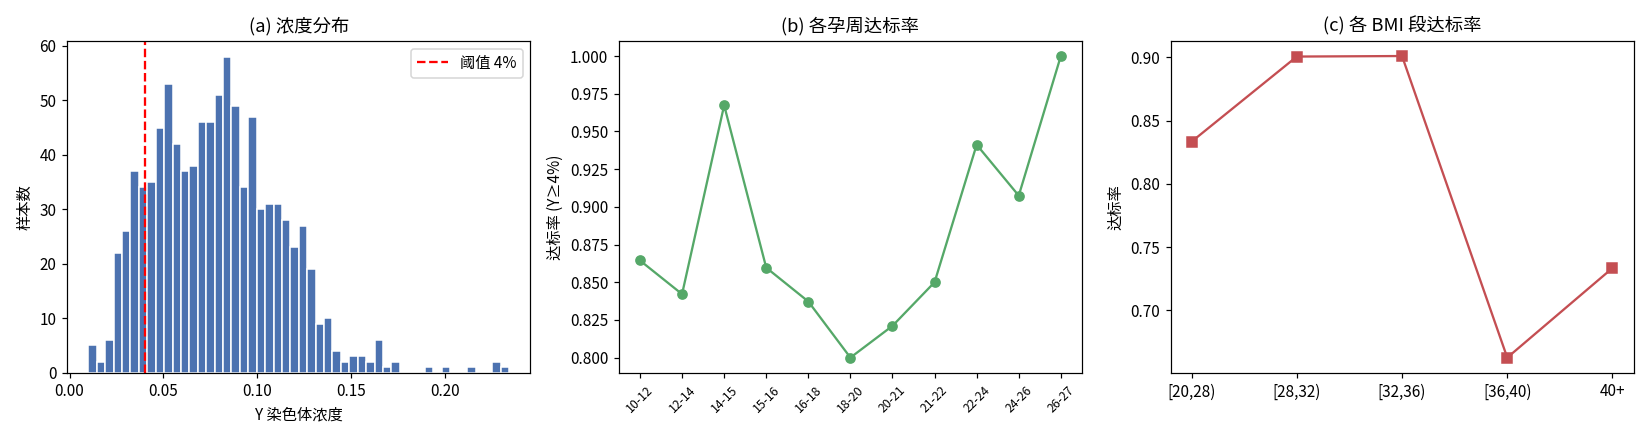
\includegraphics[width=0.92\textwidth]{fig1_dist.png}
\caption{男胎浓度分布及分孕周、分 BMI 段的达标率}\label{fig:dist}
\end{figure}

\begin{figure}[H]
\centering
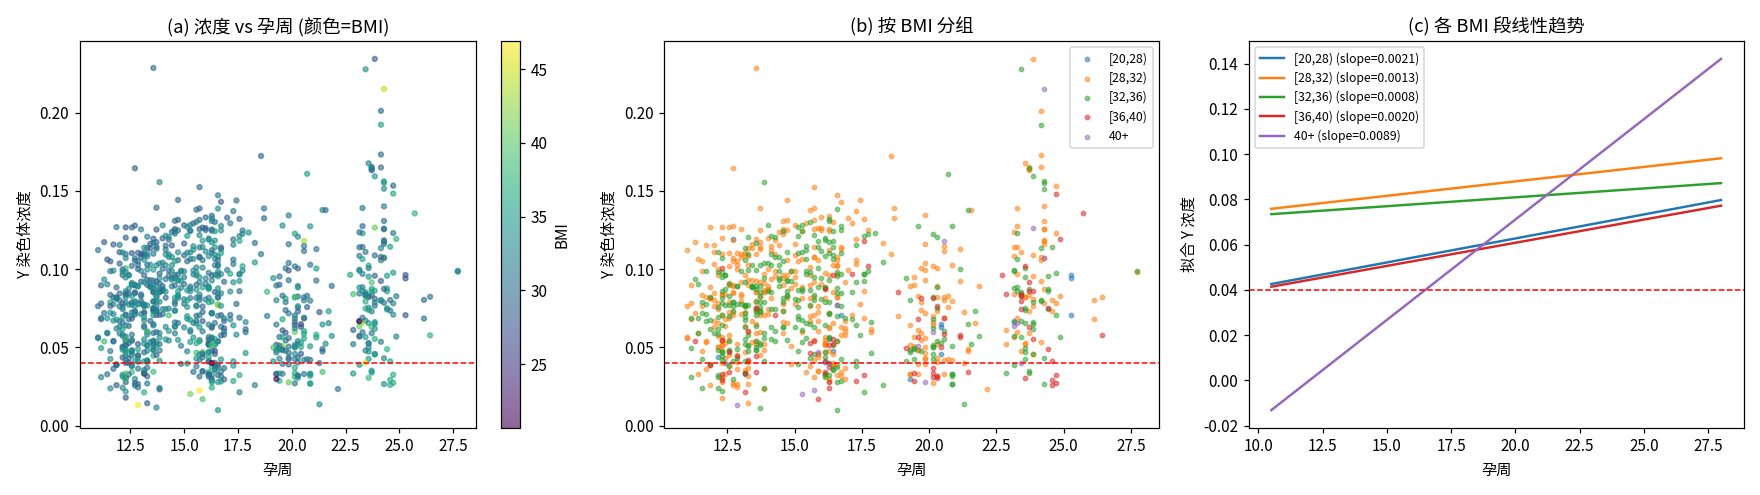
\includegraphics[width=0.98\textwidth]{fig2_trend.png}
\caption{浓度--孕周散点（颜色为 BMI）及各 BMI 段线性趋势}\label{fig:trend}
\end{figure}

\begin{figure}[H]
\centering
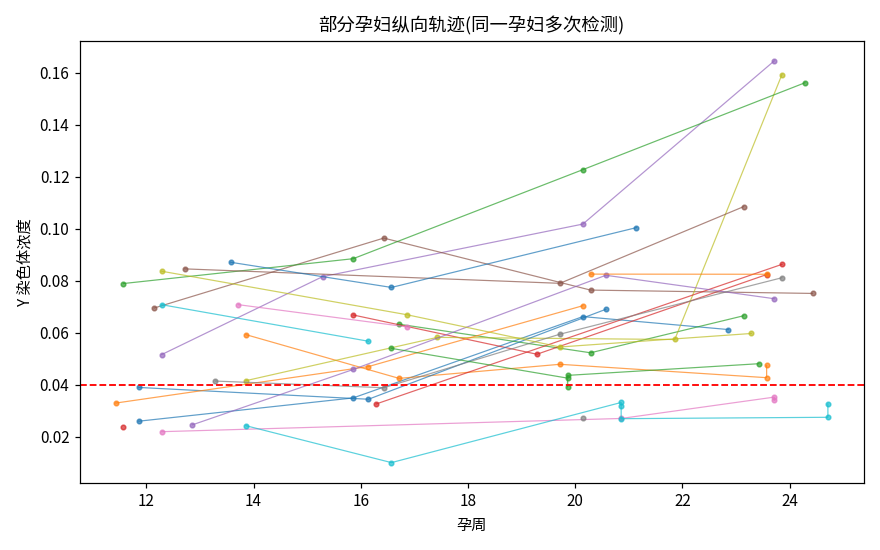
\includegraphics[width=0.75\textwidth]{fig3_traj.png}
\caption{部分孕妇的纵向检测轨迹（同一孕妇多次检测）}\label{fig:traj}
\end{figure}

\begin{figure}[H]
\centering
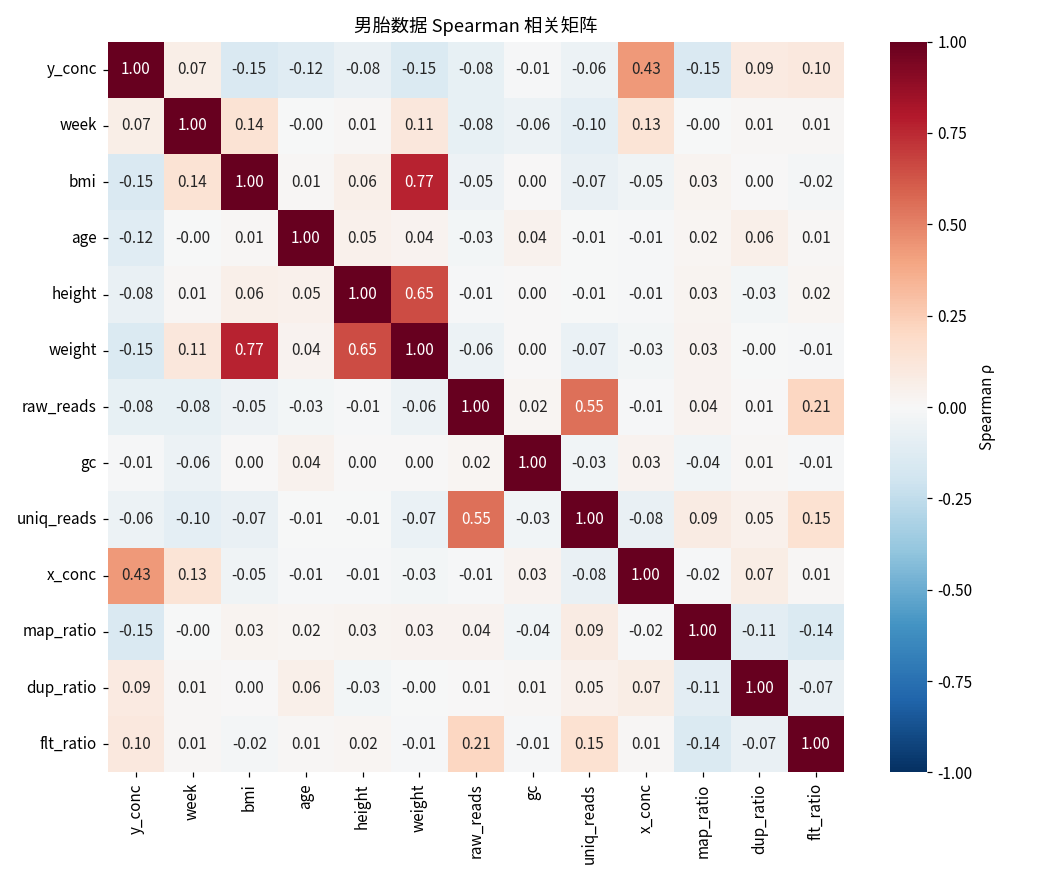
\includegraphics[width=0.8\textwidth]{fig4_corr.png}
\caption{主要变量 Spearman 相关矩阵}\label{fig:corr}
\end{figure}

%============================================================
\section{问题一：Y 染色体浓度与孕周、BMI 的相关特性与关系模型}
\subsection{相关性分析}
对 Y 浓度与各连续指标计算 Pearson 与 Spearman 相关（行级 $n=1081$），并对同一孕妇取均值计算个体级相关（$n=267$），结果见表 \ref{tab:corr}。GC 含量与浓度无相关（$p=0.5$），说明其属于质控指标而非浓度的决定因素。

\begin{table}[H]
\centering\small
\caption{Y 染色体浓度与各指标的相关性}\label{tab:corr}
\begin{tabular}{lcccc}
\toprule
指标 & 行级 Pearson $r$ & $p$ 值 & 行级 Spearman $\rho$ & 个体级 Spearman $\rho$\\
\midrule
孕周 & $+0.124$ & $4\times10^{-5}$ & $+0.082$ & ---\\
BMI & $-0.152$ & $5\times10^{-7}$ & $-0.156$ & $-0.199$（$p=0.001$）\\
体重 & $-0.180$ & $2\times10^{-9}$ & $-0.167$ & $-0.219$（$p<0.001$）\\
年龄 & $-0.120$ & $8\times10^{-5}$ & $-0.118$ & $-0.127$（$p=0.038$）\\
身高 & $-0.104$ & $6\times10^{-4}$ & $-0.100$ & $-0.129$（$p=0.035$）\\
原始读段数 & $-0.111$ & $3\times10^{-4}$ & $-0.087$ & ---\\
\bottomrule
\end{tabular}
\end{table}

行级相关受"高 BMI 者更晚受检"的混杂影响；孕周的真实效应需由组内估计给出（见下节）。

\subsection{关系模型：线性混合效应模型}
\textbf{模型设定}。孕妇 $i$ 的第 $j$ 次检测（孕周 $t_{ij}$）浓度 $y_{ij}$ 满足
\begin{equation}
y_{ij}=(\beta_0+u_{0i})+(\beta_1+u_{1i})(t_{ij}-11)+\beta_2(\mathrm{BMI}_i-32.3)+\varepsilon_{ij},
\label{eq:lmm}
\end{equation}
\begin{equation}
\begin{bmatrix}u_{0i}\\u_{1i}\end{bmatrix}\sim N(\mathbf{0},\Sigma),\qquad
\varepsilon_{ij}\sim N(0,\sigma^2),
\label{eq:lmm-re}
\end{equation}
其中 $u_{0i}$（随机截距）刻画个体浓度水平差异，$u_{1i}$（随机斜率）刻画个体增长速率差异；以"孕周$-11$"与"BMI$-32.3$"中心化，使截距可解释为孕 11 周、平均 BMI 处的预测浓度。

\textbf{模型比较与显著性检验}（表 \ref{tab:aic}，全部 ML 估计）：随机截距相对普通回归的似然比 $\mathrm{LR}=7.1$（$p=0.008$）；随机斜率相对仅随机截距 $\mathrm{LR}=163.6$（$p\approx3\times10^{-36}$）——个体间不仅水平不同，增长速率亦显著不同。

\begin{table}[H]
\centering\small
\caption{候选模型 AIC/BIC 比较}\label{tab:aic}
\begin{tabular}{lcc}
\toprule
模型 & AIC & BIC\\
\midrule
OLS：$y\sim week$ & $-4287.5$ & $-4277.5$\\
OLS：$y\sim week+bmi$ & $-4318.6$ & $-4303.6$\\
LMM（随机截距） & $-5053.6$ & $-5028.7$\\
LMM（随机截距$+$随机斜率） & $\mathbf{-5213.2}$ & $\mathbf{-5178.3}$\\
\bottomrule
\end{tabular}
\end{table}

\textbf{最终模型参数（REML）}：$\hat\beta_0=0.0586$（SE $0.0020$，$t=29.7$）；$\hat\beta_1=0.0035$（SE $0.0002$，$t=14.5$，$p<10^{-4}$）；$\hat\beta_2=-0.0012$（SE $0.0005$，$t=-2.27$，$p=0.023$）。方差分量 $\hat\sigma_u^2=7.9\times10^{-4}$、$\hat\sigma_s^2=6.0\times10^{-6}$、$\hat\sigma^2=1.86\times10^{-4}$。

\textbf{三点解读}：
\begin{enumerate}
\item 孕周每增加 1 周，同一孕妇浓度平均上升 $0.35$ 个百分点（孕 11$\to$23 周约 $+4.2$ 个百分点），且个体斜率变异显著（$\hat\sigma_s^2>0$）；
\item 校正孕周后，BMI 每高 1 个单位，浓度水平平均低约 $0.12$ 个百分点（$p=0.023$），与临床"母体肥胖降低胎儿分数"的机制一致；
\item 组内相关系数 $ICC=\sigma_u^2/(\sigma_u^2+\sigma_s^2+\sigma^2)=0.81$：约 $81\%$ 的随机变异来自孕妇间的水平差异——个体"标签"远强于时间与体质效应，这解释了行级相关为何微弱，也说明对所有人采用同一时点必然使部分个体"过早"或"过晚"（问题二的建模前提）；条件 $R^2=0.842$（边际 $R^2=0.166$）。
\end{enumerate}

\textbf{稳健性与诊断}：加入年龄后 $\hat\beta_2$ 不变（$p=0.023$）而年龄自身不显著（$p=0.24$）；标准化残差均值约 0、标准差约 0.81（个体内相关所致），轻度厚尾（Shapiro $W=0.95$，大样本易拒绝正态），不影响混合模型估计一致性；BLUP 个体水平 $u_0$ 的范围为 $[-0.052,0.117]$（p5--p95），见图 \ref{fig:blup}。

\subsection{达标概率的 logit 模型}
以是否达标（$y\ge4\%$）为响应：
\begin{equation}
\ln\frac{p}{1-p}=1.68+0.042(t-11)-0.122(\mathrm{BMI}-32.3)-0.045(a-29).
\label{eq:logit}
\end{equation}
BMI 系数显著（$p<10^{-4}$，每单位 OR$\approx0.885$），年龄边际显著（$p=0.06$），而孕周项在行级不显著（$p=0.07$）——再次体现截面混杂。因此"达标率--孕周"曲线由式 \eqref{eq:logit} 仅作示意，组别层面的达标分布一律以式 \eqref{eq:lmm}--\eqref{eq:lmm-re} 的个体达标时间 $\tau$ 表示（见 6.1 节），不同 BMI 的达标概率曲线与等值线见图 \ref{fig:passprob} 与图 \ref{fig:contour}。

\begin{figure}[H]
\centering
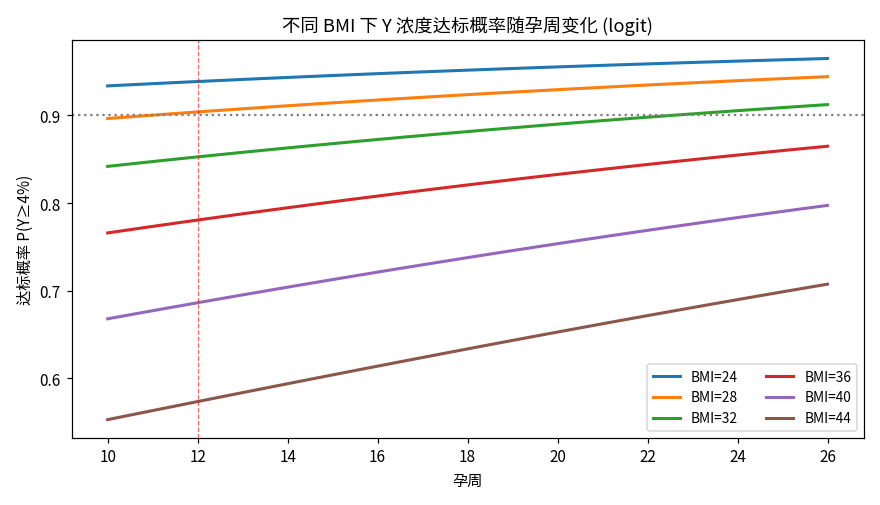
\includegraphics[width=0.78\textwidth]{fig5_passprob.png}
\caption{不同 BMI 下达标概率随孕周变化（logit 模型）}\label{fig:passprob}
\end{figure}

\begin{figure}[H]
\centering
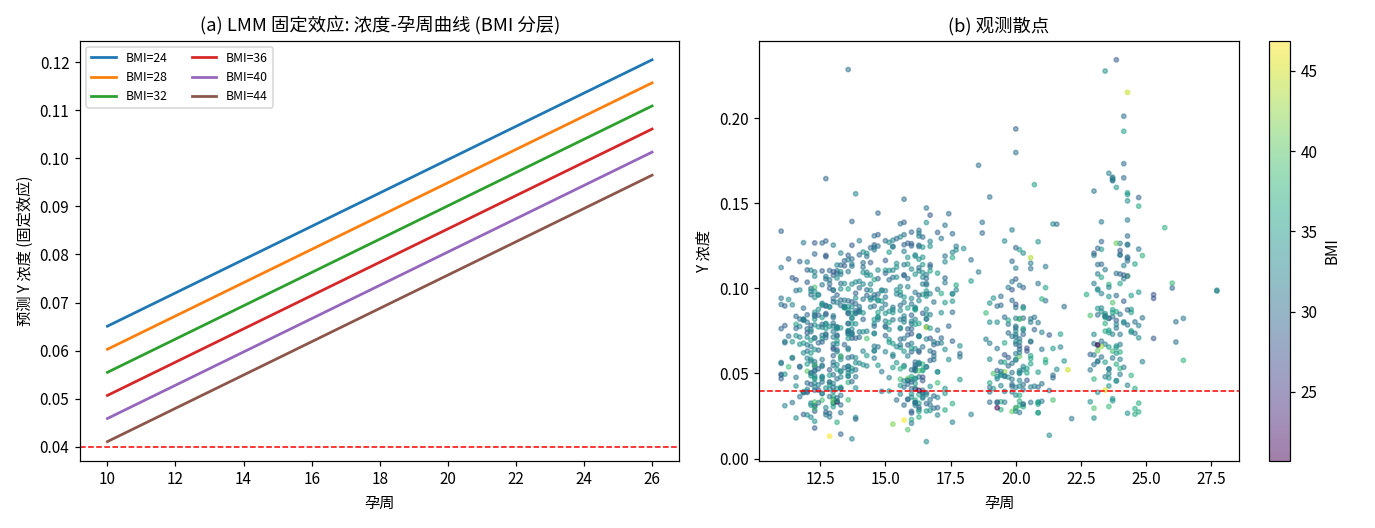
\includegraphics[width=0.98\textwidth]{fig6_surface.png}
\caption{(a) LMM 固定效应预测的浓度--孕周曲线（BMI 分层）；(b) 观测散点}\label{fig:surface}
\end{figure}

\begin{figure}[H]
\centering
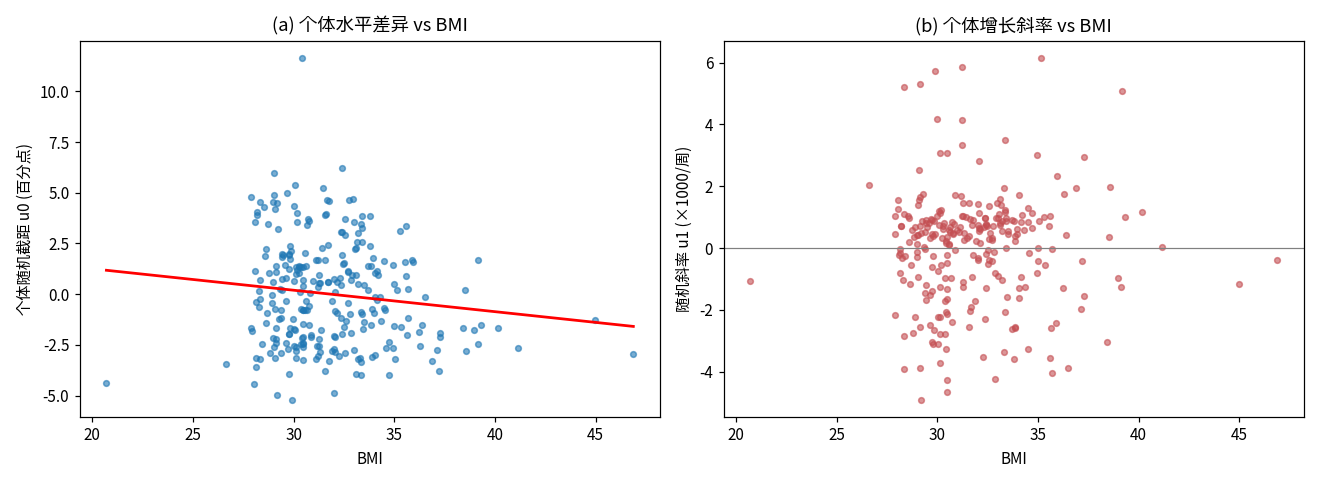
\includegraphics[width=0.98\textwidth]{fig7_blup.png}
\caption{个体随机效应（水平 $u_0$ 与斜率 $u_1$）与 BMI 的关系}\label{fig:blup}
\end{figure}

\begin{figure}[H]
\centering
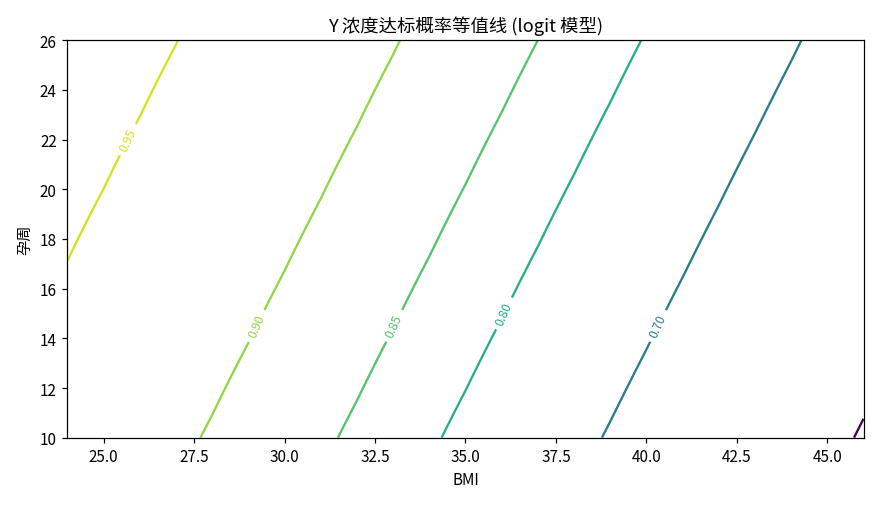
\includegraphics[width=0.78\textwidth]{fig8_contour.png}
\caption{Y 浓度达标概率等值线（孕周$\times$BMI）}\label{fig:contour}
\end{figure}

\noindent\textbf{问题一小结}：Y 浓度与孕周显著正相关（组内 $0.0035$/周，$p<10^{-4}$）、与 BMI/体重显著负相关（$p<0.05$）；随机截距+随机斜率的 LMM 刻画良好（条件 $R^2=0.84$），参数检验、嵌套检验与残差诊断均通过；$ICC=0.81$ 说明个体差异主导，为后续分组与个体化时点决策提供统计依据。

%============================================================
\section{问题二：基于 BMI 分组的最佳 NIPT 时点决策}
\subsection{个体最早达标时间 $\tau$ 的估计}
\textbf{BLUP 法}：以式 \eqref{eq:lmm} 的随机效应 BLUP $\hat u_{0i},\hat u_{1i}$ 反解 $\tau_i$：
\begin{equation}
\hat\tau_i=11+\frac{0.04-\bigl[\hat\beta_0+\hat u_{0i}+\hat\beta_2(\mathrm{BMI}_i-32.3)\bigr]}{\hat\beta_1+\hat u_{1i}},\qquad
\hat\tau_i\in[10,30].
\label{eq:tau}
\end{equation}
\textbf{插值法（对照）}：对每名孕妇按时间排序，在跨越 $4\%$ 的相邻两次检测间线性插值（首测即达标者按总体斜率外推）。两法估计高度一致（$n=260$，Spearman $\rho=0.731$，中位差 0.00 周），估计稳健。

$\tau$ 分布特征：约 $66\%$ 的孕妇 11 周前即可达标，中位 10（受窗口下限截断），P75$=12.5$，P90$\approx22.8$；约 $5\%$ 的孕妇 25 周仍难达标（$\tau>25$）。按 BMI 分组（图 \ref{fig:tauhist}、\ref{fig:taubmi}）：BMI$<36$ 各组分布几乎相同（中位 10、P75$\approx11.3$--$12.0$），BMI$\ge36$ 组整体右移（中位 14.2、P75$=17.9$、P90$\approx21.0$）。

\subsection{风险函数与优化判据}
\textbf{风险权重}：按题意"12 周内低风险、13--27 周高风险、28 周后极高风险"，将三级风险 $1:4:16$ 平滑为
\begin{equation}
w(t)=e^{k(t-11)},\qquad k=\frac{\ln4}{9},\qquad
w(11)=1,\ w(20)=4,\ w(29)=16.
\label{eq:w}
\end{equation}
\textbf{发现孕周}：孕妇 $i$ 在时点 $t$ 首检，若 $t\ge\tau_i$ 则一次可靠检出（发现孕周 $=t$）；否则检测失败、复查后需至 $\tau_i+\Delta$ 才能可靠检出：
\begin{equation}
d_i(t)=\begin{cases}t, & t\ge\tau_i,\\ \tau_i+\Delta, & t<\tau_i.\end{cases}
\label{eq:d}
\end{equation}
\textbf{组期望风险} $R_g(t)=\E_{i\in g}[w(d_i(t))]$。异常发生率 $q$ 为公共乘性常数，不进入 $\arg\min$（假设 5）。

\textbf{双目标判据}：数值分析显示（见 6.4 灵敏度），$R_g(t)$ 从窗口起点到某拐点几乎平坦——因为"提前检测失败而后复查"的期望发现孕周与"在拐点前推迟首检"接近。纯风险最小化因此会把所有组推向窗口下限 10 周，导致 30\%--90\% 的孕妇需要复检。故采用"风险平带约束 $+$ 单次达标率最大化"：
\begin{equation}
t^{*}=\arg\max_{t}\bigl\{P(\tau\le t):\ R_g(t)\le 1.02\,R_g^{\min}\bigr\},
\label{eq:obj}
\end{equation}
即在期望风险不超过最小方案 $2\%$ 的前提下，取单次通过率最高（复检负担最小、依从性最好）的时点。两种判据结果同时报告。

\subsection{BMI 合理分组}
\textbf{候选分档方案比较}（表 \ref{tab:part}，$\Delta=1.5$ 周，最小组成员数 $n_{\min}=10$）。

\begin{table}[H]
\centering\small
\caption{各分档方案的组最优时点与加权平均风险（推荐判据式 \eqref{eq:obj}）}\label{tab:part}
\resizebox{\textwidth}{!}{%
\begin{tabular}{lcccccc}
\toprule
方案 & 组（人数） & 风险最小时点 & 平带推荐时点 & 推荐时点达标率 & 加权平均风险$^{*}$\\
\midrule
统一（不分组） & 全体（267） & 10.0 & 10.5 & 65\% & 2.343\\
\multirow{5}{*}{题示五档} & $[20,28)$（5）$^{\dagger}$ & --- & --- & --- & \multirow{5}{*}{2.275}\\
 & $[28,32)$（147） & 10.0 & 10.5 & 69\% &\\
 & $[32,36)$（95） & 10.0 & 10.5 & 70\% &\\
 & $[36,40)$（16） & 10.0 & 14.3 & 56\% &\\
 & $[40,\infty)$（4）$^{\dagger}$ & --- & --- & --- &\\
\multirow{4}{*}{四档（低端合并）} & $[20,32)$（152） & 10.0 & 10.5 & 68\% & \multirow{4}{*}{2.301}\\
 & $[32,36)$（95） & 10.0 & 10.5 & 70\% &\\
 & $[36,40)$（16） & 10.0 & 14.3 & 56\% &\\
 & $[40,\infty)$（4）$^{\dagger}$ & --- & --- & --- &\\
\multirow{3}{*}{三档} & $[20,32)$（152） & 10.0 & 10.5 & 68\% & \multirow{3}{*}{2.348}\\
 & $[32,36)$（95） & 10.0 & 10.5 & 70\% &\\
 & $[36,\infty)$（20） & 10.0 & 14.5 & 55\% &\\
\bottomrule
\end{tabular}}
\\[-4pt]
{\footnotesize $^{\dagger}$样本不足 10 人，独立估计不可靠，按稳健性原则并入邻组；$^{*}$为推荐时点下按人数加权的平均风险。风险最小基准下各方案最优时点均落在 10--10.5 周附近，统一与分档期望风险差异很小（2.305 vs 2.23--2.26），分组收益主要体现在单次达标率与复检负担上（见表 \ref{tab:policy}）。}
\end{table}

\textbf{组间差异检验}：三档组间 $\tau$ 的 Kruskal--Wallis $H=29.8$（$p=3.4\times10^{-7}$）；两两 Mann--Whitney：$[20,32)$ vs $[32,36)$ 的 $p=0.78$（无差异），$[32,36)$ vs $[36,\infty)$ 的 $p=1.1\times10^{-6}$，$[20,32)$ vs $[36,\infty)$ 的 $p=1.3\times10^{-7}$。\textbf{结论：BMI=36 是数据中唯一显著分界；32 附近无可辨差异，$[20,32)$ 与 $[32,36)$ 可合并或仅作服务分层}。

\textbf{数据驱动分界点联合搜索}：对 $k=1,2$ 个分界在 $[28,46]$ 以 0.5 步长扫描（目标为分档推荐时点下的加权风险，每组 $\ge10$ 人）：$k=1$ 最优分界 29.0（2.340，与统一基准 2.343 几乎持平）；$k=2$ 最优 $[29.5,33.5]$（2.334）——分界位置随随机波动漂移且增益不超过 $0.35\%$，再次印证"36 以下无实质分组价值、36 以上应单独成组"。经验五档中 $[20,28)$（5 人）与 $[40,\infty)$（4 人）样本过少，合并是必要的数据驱动修正。

\textbf{推荐分组}：主方案两档，\textbf{G1：BMI$\in[20,36)$；G2：BMI$\ge36$}；如临床需要服务分层，可执行三档（在 32 处分流，时点不变）。

\subsection{各组最佳时点与策略对比}
按式 \eqref{eq:obj}：G1 推荐首检 $t=11.0$ 周（风险平带约 $[10,\ 10.5$--$12.8]$，考虑临床排期取整，11 周为数据观测起点且在"12 周内低风险"区）；G2 推荐 $t=14.5$ 周（14--15 周）：该组若在 10 周首检，单次通过率仅约 10\%--13\%，绝大多数孕妇需 1--3 次复检，检测失败与依从性风险高。三种策略的整体对比见表 \ref{tab:policy}（含"复检机制下的人均抽血次数"与"发现孕周分布"两类工程化指标）。

\begin{table}[H]
\centering\small
\caption{三种策略对比（BLUP 估计 $\tau$，全体 267 名孕妇）}\label{tab:policy}
\resizebox{\textwidth}{!}{%
\begin{tabular}{lcccccc}
\toprule
策略 & 平均期望风险 & 单次达标率 & 人均抽血次数 & 发现$\le12$周 & 13--27 周 & $\ge28$ 周\\
\midrule
A1：统一 10.5 周 & \textbf{2.255} & 64.8\% & 1.95 & 64.8\% & 30.7\% & 4.5\%\\
A2：统一 11 周 & 2.299 & 66.7\% & 1.86 & 66.7\% & 28.8\% & 4.5\%\\
\textbf{B：G1@11 周，G2@14.5 周} & 2.304 & \textbf{70.1\%} & \textbf{1.77} & 65.9\% & 29.6\% & 4.5\%\\
C：经验五档均 12 周 & 2.402 & 71.9\% & 1.71 & 71.9\% & 23.6\% & 4.5\%\\
\bottomrule
\end{tabular}}
\end{table}

对比结论：(i) 方案 B 与风险最优的 A1 几乎持平（$+2.2\%$），但单次达标率提高 5.3 个百分点、人均抽血从 1.95 降至 1.77 次；(ii) 经验方案 C 的期望风险比方案 B 高约 $4.3\%$（其 G2 组在 12 周仅 15\% 一次通过、人均抽血 2.97 次），说明"机械统一早检"在风险与可操作性上均不占优；(iii) 约 $4.5\%$ 的孕妇（$\tau\ge28$，多为 BMI$\ge36$ 且浓度长期偏低者）在任何单一时点策略下都难在窗口内可靠检出，须以个体化随访兜底（问题三）。

\begin{figure}[H]
\centering
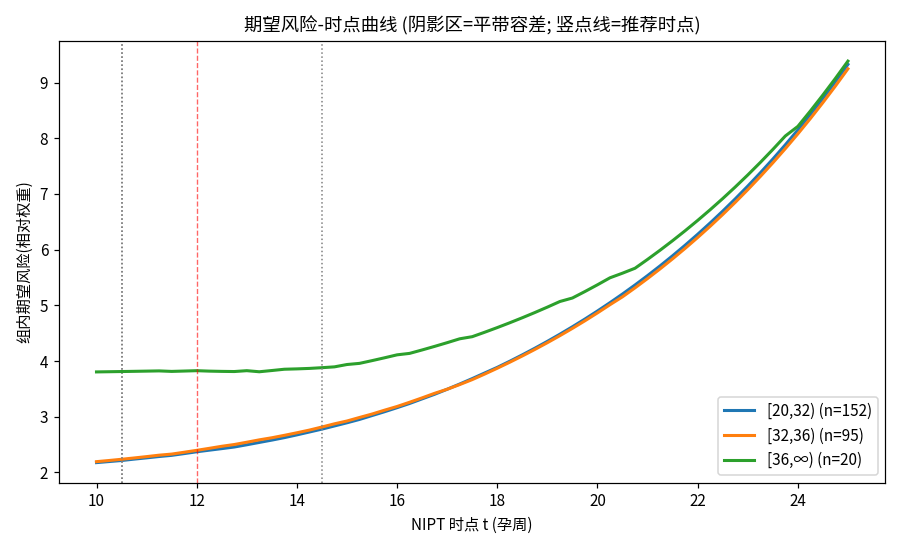
\includegraphics[width=0.85\textwidth]{fig9_riskcurve.png}
\caption{各组期望风险--时点曲线（竖点线为推荐时点）}\label{fig:riskcurve}
\end{figure}

\begin{figure}[H]
\centering
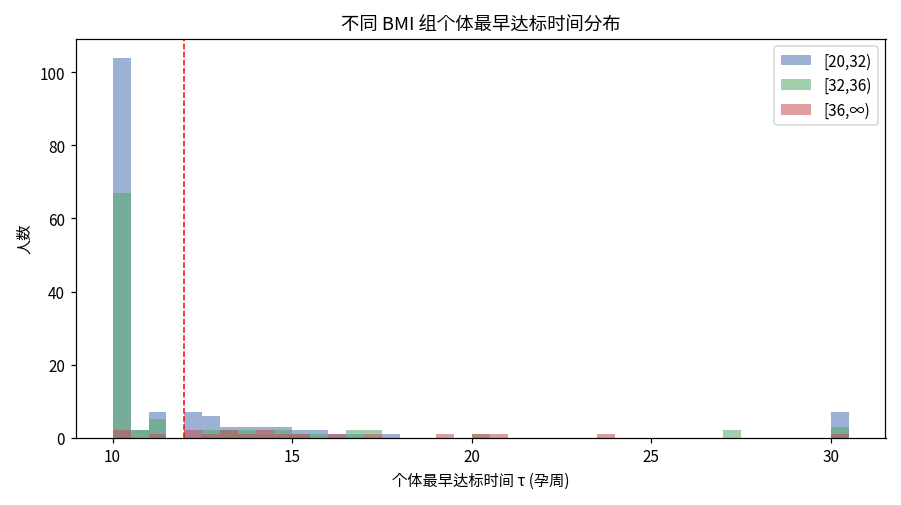
\includegraphics[width=0.85\textwidth]{fig10_tau_hist.png}
\caption{不同 BMI 组个体最早达标时间 $\tau$ 的分布}\label{fig:tauhist}
\end{figure}

\subsection{检测误差对结果的影响}
\textbf{误差来源与量化}：
\begin{enumerate}
\item \emph{浓度测量噪声}：同周重复检测估计 $\sigma_m=0.00903$，占 $4\%$ 阈值的 $22.6\%$；由斜率 $1/\hat\beta_1\approx286$ 周/单位浓度换算，$\tau$ 的标准不确定度约 $\sigma_m/0.0035\approx2.6$ 周；
\item \emph{复查延迟} $\Delta$（临床排期，0.5--3 周）；
\item \emph{风险斜率设定} $k$（$\pm15\%$）。
\end{enumerate}
\textbf{参数自助}（400--600 次，按孕妇重抽样并对 $\tau$ 注入测量噪声，$\Delta$ 在 0.5--3 间均匀取值，$k$ 扰动 $\pm15\%$）：
G1 推荐时点中位 11.3 周（95\% 区间 $[10.5,12.8]$）；G2 中位 13.4 周（95\% 区间 $[11.0,16.0]$）。$\Delta$ 单因子敏感性：G2 由 $\Delta=0.5$ 时的 13.0 周单调升至 $\Delta=3$ 时的 15.5 周，G1 稳定于 10.2--10.5 周。故 G1 的推荐在误差下非常稳健，G2 存在约 $\pm2.5$ 周的合理区间，取 14.5 周居中稳健。

\noindent\textbf{问题二小结}：推荐的合理分组为 BMI$<36$ 与 BMI$\ge36$（执行三档时 $[20,32)$ 与 $[32,36)$ 同策），首检时点分别约 11 周与 14.5 周；相对经验统一 12 周方案，期望风险降低约 $4\%$，同时兼顾单次达标率、复检负担与个体差异；误差分析表明结论稳健。

%============================================================
\section{问题三：多因素、达标比例与检测误差下的分组时点优化}
\subsection{多因素模型：身高、体重、年龄的增量信息}
在式 \eqref{eq:lmm} 上逐步加入年龄、身高、体重（均为组内中心化），模型比较见表 \ref{tab:multi}。似然比检验：加年龄 $\mathrm{LR}=1.40$（$p=0.24$）；再加身高体重 $\mathrm{LR}=2.08$（$p=0.15$），均不显著；AIC 不再下降（F4 $-5211.8$ vs F1 $-5213.2$），BIC 同样不支持。全协变量模型中体重/BMI 因共线性吸收而单项不显著，但个体级分析（表 \ref{tab:corr}）表明体重确与浓度负相关。孕周$\times$BMI 交互项使 AIC 略降（F5 $=-5217.8$）但 BIC 反升（$-5163.0$ vs $-5178.3$），且各 BMI 段组内斜率几乎相同（5.2 节），交互效应量微小，按简约原则不采纳。

\begin{table}[H]
\centering\small
\caption{多因素线性混合模型比较（ML）}\label{tab:multi}
\begin{tabular}{lcccc}
\toprule
模型 & 固定效应 & AIC & BIC & LL\\
\midrule
F1 & 孕周+BMI & $\mathbf{-5213.2}$ & $\mathbf{-5178.3}$ & 2613.6\\
F2 & $+$年龄 & $-5212.6$ & $-5172.7$ & 2614.3\\
F3 & $+$身高$+$体重 & $-5212.6$ & $-5167.8$ & 2615.3\\
F4 & $+$全部 & $-5211.8$ & $-5161.9$ & 2615.9\\
F5 & F4$+$孕周$\times$BMI & $-5217.8$ & $-5163.0$ & 2619.9\\
\bottomrule
\end{tabular}
\end{table}

\textbf{对个体达标时间的解释力}：对未受窗口截断影响的子样本（$10.4<\tau<28$，$n=85$）回归，$\tau\sim\mathrm{BMI}$ 的 $R^2=0.081$；加入年龄/身高/体重后 $R^2=0.118$（adj.\ $R^2=0.074$）。对孕周校正后的个体浓度水平，多因素仅使 $R^2$ 由 0.053 增至 0.081。未截断子样本上 $\tau$ 与 BMI/体重/年龄的 Spearman 相关为 $0.27/0.26/0.24$（$p<0.05$），身高不显著。

\textbf{结论}：达标时间的主体差异是个体性的（LMM 随机效应），BMI 抓住了其中可解释的主要部分，身高/体重/年龄只提供少量增量——维持 BMI 分档既简洁又统计充分。多因素的用途在于\textbf{组内个体预警}：若某孕妇的个体化预测 $\hat\tau_i$ 显著晚于组内时点（例如 BMI 属 G1 但体重极大、$\hat\tau_i$ 接近 14 周），应为其安排更晚的首检或个体化随访。

\subsection{达标比例--风险权衡}
"达标比例"（单次检测时浓度 $\ge4\%$ 的孕妇比例）直接度量临床可操作性。在约束 $P(\tau\le t)\ge p_0$ 下求风险最小时点，结果见表 \ref{tab:trade} 与图 \ref{fig:trade}。

\begin{table}[H]
\centering\small
\caption{达标比例约束 $p_0$ 下的最优时点与对应期望风险（周数/风险权重）}\label{tab:trade}
\begin{tabular}{lcc}
\toprule
约束 $p_0$ & G1（BMI$<36$） & G2（BMI$\ge36$）\\
\midrule
无约束（风险最小） & 10.0 / 2.18 & 10.0 / 3.81\\
$\ge0.70$ & 11.0 / 2.27 & 16.2 / 4.14\\
$\ge0.80$ & 12.8 / 2.47 & 19.5 / 5.13\\
$\ge0.90$ & 15.2 / 2.97 & 20.8 / 5.67\\
$\ge0.95$ & 20.5 / 5.18 & 24.0 / 8.21\\
\bottomrule
\end{tabular}
\end{table}

可见\textbf{风险与达标率存在明确权衡}：G2 若强求单次达标率 $90\%$，时点需推迟到约 21 周，期望风险上升约 $49\%$（21 周已属中期，阳性者治疗窗口大幅缩短）；G1 在 $0.9$ 约束下时点 15.2 周也显著劣于 11 周。故"达标比例"应作为约束而非单目标。本文推荐工作点：G1 取 $p_0\approx0.71$（11 周）、G2 取 $p_0\approx0.55$（14.5 周），即 6.4 节方案 B：以"复检机制兜底低达标比例"，换取尽量早的可靠首检；若机构偏好更高的单次通过率，可按表 \ref{tab:trade} 查表取值并承担相应风险增量。

\begin{figure}[H]
\centering
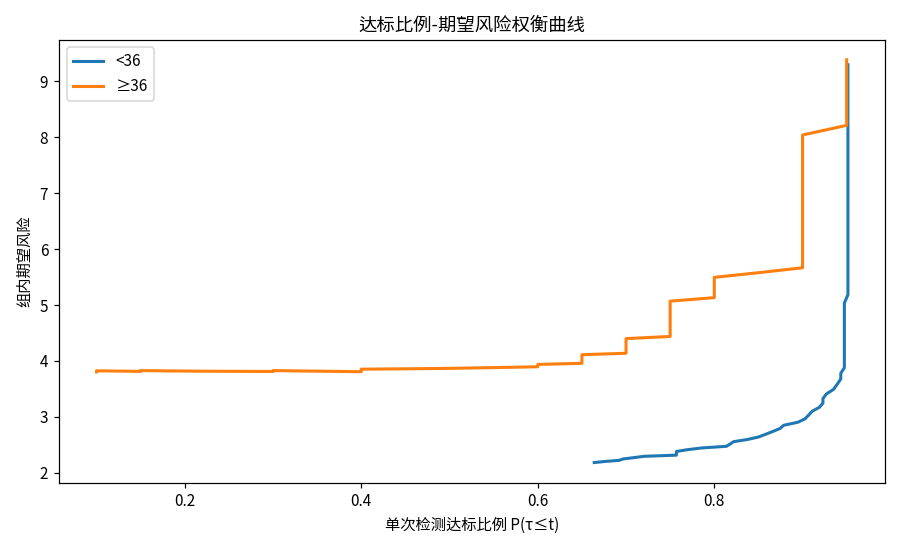
\includegraphics[width=0.85\textwidth]{fig11_tradeoff.png}
\caption{达标比例--期望风险权衡曲线（G1/G2）}\label{fig:trade}
\end{figure}

\begin{figure}[H]
\centering
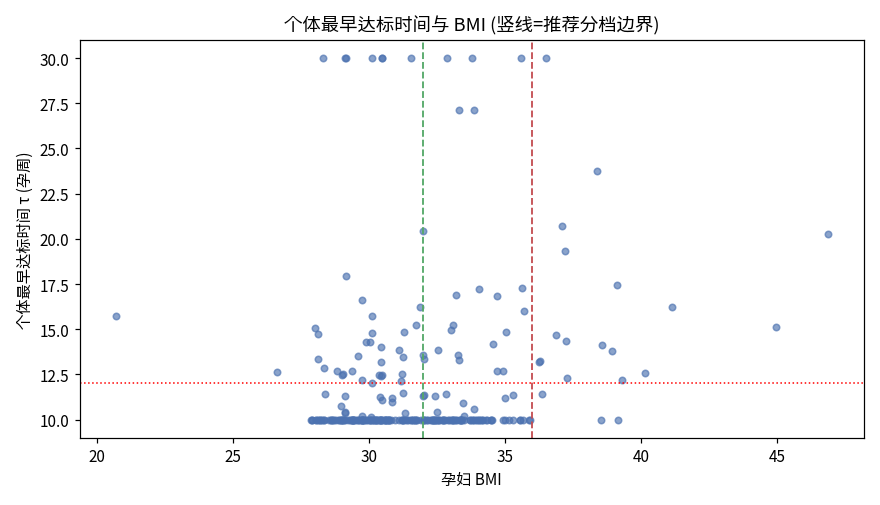
\includegraphics[width=0.85\textwidth]{fig12_tau_bmi.png}
\caption{个体最早达标时间与 BMI（竖线为推荐分界 32/36）}\label{fig:taubmi}
\end{figure}

\subsection{检测误差对分组与时点的影响}
\textbf{误差传播}（参数自助 600 次：按孕妇重抽样，浓度噪声注入 $\tau$，另叠加到检执行偏差 $\varepsilon\sim N(0,0.5^2)$ 周）：
G1 推荐时点中位 11.3 周（95\% 区间 $[10.8,11.5]$），执行偏差使期望风险平均上升约 $7.1\%$；G2 推荐时点中位 13.4 周（95\% 区间 $[11.5,15.8]$），执行偏差风险增幅仅约 $1.7\%$（该组风险主要由 $\tau$ 的不可服务尾部决定，对时点小扰动不敏感）。

\textbf{分界点 $\pm1$ 的稳健性}：分界取 35/36/37 时，低侧推荐时点均为 10.5 周，高侧分别为 12.0/14.5/13.3 周；三处分界两侧 $\tau$ 差异的 Mann--Whitney $p<10^{-5}$。即分界取 36 附近任意值都能将"需晚检"群体分离，分组结论稳健。

\noindent\textbf{问题三小结}：年龄/身高/体重等因素的增量信息有限（LMM 检验不显著、$R^2\le0.12$），BMI 分档简洁且统计充分；给出达标比例 $0.70$--$0.95$ 约束下的权衡表与推荐工作点；测量噪声（约 $\tau$ 的 2.6 周）与执行偏差对 G1 时点影响小（自助区间宽约 1 周）、对 G2 更小。

%============================================================
\section{问题四：女胎染色体非整倍体判定方法}
\subsection{问题设定与数据核查}
以女胎 AB 列标注（13/18/21 号染色体非整倍体，含组合型）为判定金标准：异常行 67/605（11.1\%），异常孕妇 44/147（29.9\%）。特征集共 17 维：三条常染色体 Z 值 $z_{13},z_{18},z_{21}$；X 染色体 Z 值与浓度 $z_X,c_X$（并加入 $c_X^2$ 捕捉其负值深度信息）；总 GC 与各染色体 GC 含量；原始/唯一读段数与比对、重复、过滤比例；BMI、年龄、孕周。

数据核查发现三个重要事实（决定建模路线）：
\begin{enumerate}
\item \emph{单条记录的 Z 值规则与标签严重脱节}：T13/T18/T21 阳性行的对应染色体 $z>3$ 占比仅 $4\%/0\%/0\%$，而阴性行中分别有 18/33/0 行 $z>3$；
\item \emph{同孕妇多次检测标签不一致率达 29.3\%}（43/147），个别孕妇不同孕周记录标出不同三体（如 B004 的第 3 行标 T21、第 4 行标 T13）；
\item 阳性组与阴性组在多数质量指标（GC、过滤比、比对率、读段数）上的中位数几乎重合。
\end{enumerate}

因此不能采用"单条记录 $z>3$ 即判阳"的教科书规则，必须：(a) 借助多特征联合判别提取弱信号；(b) 以质控门控剔除低质量记录；(c) 以多胎次证据整合（复检）抑制假阳性。这与临床"低风险报告 $\to$ 高风险复核 $\to$ 侵入性产前诊断确认"的三级流程一致。

\subsection{方法：QC 门控 + 判别模型 + 概率校准 + 多胎次整合}
\begin{enumerate}
\item \textbf{QC 门控}：GC$\in[0.40,0.60]$、比对率 $\ge0.70$、重复率 $\le0.30$、唯一比对读段 $\ge200$ 万；数据中 63.4\% 记录通过。阳性占比在通过/未通过样本间接近（11.5\% vs 10.4\%），说明 QC 主要反映测序质量而非患病状态，作为"样本不合格、建议重新采血"的依据。
\item \textbf{判别模型}：带类别平衡的罚逻辑回归（LR）与随机森林（RF，500 棵树）；输入为 17 维特征。\textbf{评估协议}：GroupKFold 五折、\emph{按孕妇分组}，杜绝同一孕妇多次检测的泄漏；全部评估基于折外（OOF）概率。
\item \textbf{概率校准}：类别不平衡与平衡权重使原始概率过度自信（Brier$=0.158>$基准 0.099）；对 OOF 概率拟合等渗（Isotonic）回归后 Brier 降至 0.074。
\item \textbf{孕妇级证据整合}：规则 A"任一次 $p>0.5$ 判筛查阳性"；规则 B"$\ge2$ 次独立记录 $p>0.5$ 判高风险（转诊产前诊断）"。
\end{enumerate}

\subsection{结果}
\textbf{行级判别性能}见表 \ref{tab:perf}（OOF，ROC 见图 \ref{fig:roc}）。任意非整倍体 LR AUC$=0.803$；分染色体看 T18 最强（0.832）、T13 居中（0.758）、T21 最弱（0.576，仅 13 个阳性行）。

\begin{table}[H]
\centering\small
\caption{行级判定性能（GroupKFold-5、按孕妇分组、OOF 概率）}\label{tab:perf}
\begin{tabular}{lcccc}
\toprule
目标 & 阳性行数 & LR AUC & RF AUC & LR 平均精确率（AP）\\
\midrule
任意非整倍体 & 67 & \textbf{0.803} & 0.781 & 0.441\\
T13 & 23 & 0.758 & 0.771 & 0.183\\
T18 & 46 & \textbf{0.832} & 0.796 & 0.401\\
T21 & 13 & 0.576 & 0.516 & 0.101\\
\bottomrule
\end{tabular}
\end{table}

\begin{itemize}
\item \textbf{置换检验}（100 次标签打乱、同 CV 协议）：零分布 AUC$=0.498\pm0.054$，观测 0.803，$p<0.001$——判别信号真实存在且来自特征组合；
\item \textbf{分染色体 Youden 工作点}：T13 阈值 0.157（敏感 0.87/特异 0.59）、T18 阈值 0.352（0.83/0.72）、T21 阈值 0.109（0.85/0.43）；三染色体阈值取"或"得到筛查规则：敏感性 0.94、特异性 0.30（筛查语义可接受，阳性须复核）；
\item \textbf{特征重要性}（LR 标准化系数，图 \ref{fig:coef}）：$gc_{13}$（$+1.32$）、$gc_{21}$（$-1.95$）、$c_X$（$-0.79$）、$c_X^2$（$+0.35$）、年龄（$-0.43$）、BMI（$-0.37$）、重复率（$-0.28$）、$z_{21}$（$+0.24$）、$z_{18}$（$+0.14$）——信号主要由染色体 GC 偏离、X 染色体浓度（低胎儿分数指示）与孕妇特征携带，Z 值本身贡献有限，与 8.1 节核查一致；
\item \textbf{特征消融}：去掉 X 染色体组后 AUC 降至 0.729（$-0.075$），去掉 GC 组降至 0.772（$-0.032$），去掉 Z 值组几乎不变（0.821）——再次印证信号来源；
\item \textbf{孕妇级整合}（$n=147$）：max 整合 AUC$=0.746$（自助 95\% CI $[0.665,0.831]$）、mean 整合 0.723；规则 A：敏感性 0.41、特异性 0.91、PPV 0.67；\textbf{规则 B：特异性 1.00、PPV 1.00}（数据内零假阳），敏感性 0.41——与临床一致：筛查阳性必须复核，复核阳性基本可靠；
\item \textbf{校准曲线}见图 \ref{fig:calib}；阈值 $0.2\sim0.8$ 扫描表供机构按偏好选择工作点（如阈值 0.4 时敏感性 0.79/特异性 0.69）。
\end{itemize}

\begin{figure}[H]
\centering
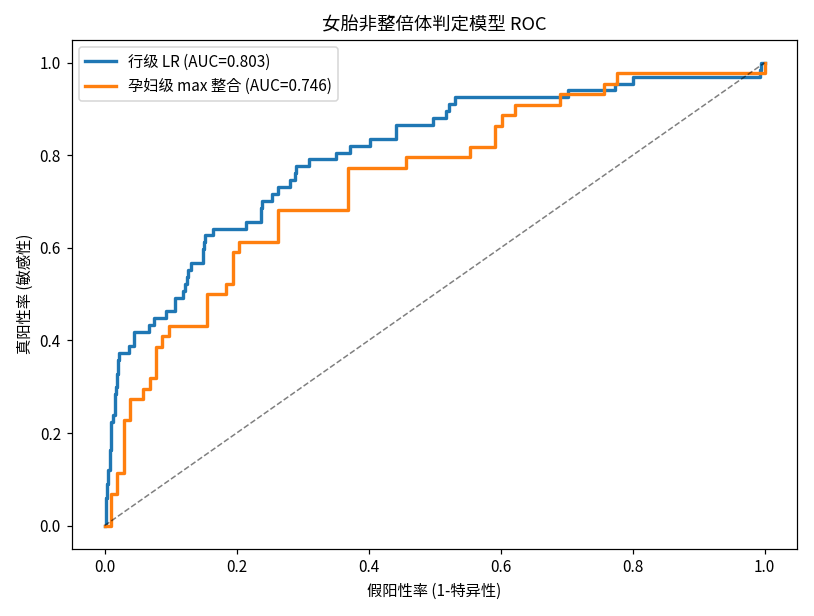
\includegraphics[width=0.72\textwidth]{fig13_roc.png}
\caption{判定模型 ROC：行级与孕妇级（max 整合）}\label{fig:roc}
\end{figure}

\begin{figure}[H]
\centering
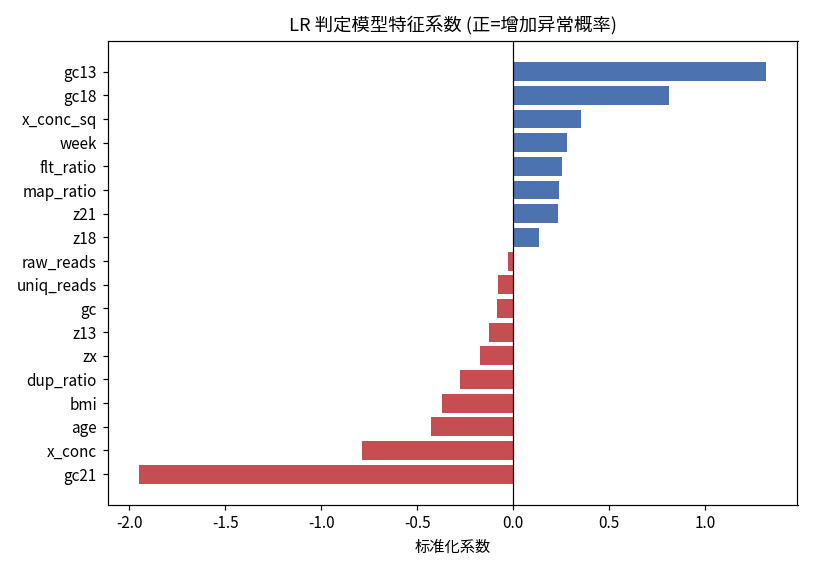
\includegraphics[width=0.78\textwidth]{fig14_coef.png}
\caption{LR 判定模型特征系数（标准化，正=增加异常概率）}\label{fig:coef}
\end{figure}

\begin{figure}[H]
\centering
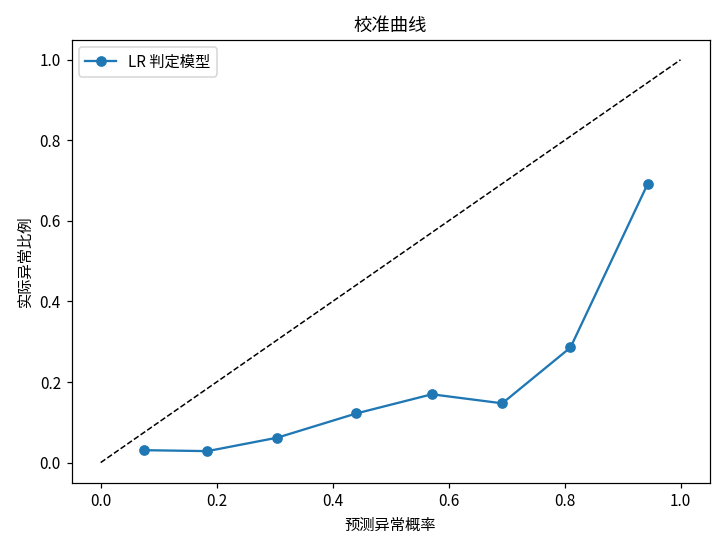
\includegraphics[width=0.68\textwidth]{fig15_calib.png}
\caption{模型校准曲线（等渗校准后）}\label{fig:calib}
\end{figure}

\subsection{推荐判定流程与误差讨论}
\textbf{女胎判定流程}：
\begin{enumerate}
\item 测序记录过 QC（GC/比对率/重复率/唯一读段），不过则判"样本不合格，建议重新采血"；
\item 合格记录计算 17 维特征并代入校准后 LR 模型，得到 $p_{13},p_{18},p_{21}$ 与综合 $p_{\max}$；
\item 综合 $p_{\max}>0.42$（Youden 工作点）判\textbf{筛查阳性}，进入复核；否则报告低风险；
\item 复核规则：同孕妇 $\ge2$ 次独立采血记录均为筛查阳性者判\textbf{高风险}，建议羊水穿刺等产前诊断确认；单次阳性者 2 周后复检；
\item T21 提示：本数据中 T21 标签可判别信号弱（AUC$\approx0.58$），该类提示应从严复核并适当增加测序深度。
\end{enumerate}

\textbf{误差与不确定性讨论}：
\begin{itemize}
\item \emph{标签噪声}：8.1 节核查表明 AB 列存在明显不一致（跨胎次标签翻转、与 Z 值规则脱节），模型性能（行级 AUC 0.80）应视为该噪声水平下"可提取信号"的下界；孕妇级规则 B 把标签噪声导致的假阳压至零；
\item \emph{类不平衡}：阳性 11.1\%，以类别平衡训练+校准处理；AP$=0.44$ 说明阳性段排名质量良好；
\item \emph{评估无乐观偏差}：交叉验证按孕妇分组、概率全部 OOF 产生；孕妇级 AUC 自助区间 $[0.665,0.831]$。
\end{itemize}

\noindent\textbf{问题四小结}：建立"QC 门控 $\to$ 多特征概率判别（LR/RF，OOF AUC 0.80）$\to$ 等渗校准 $\to$ 多胎次复核"四层判定流水线，给出综合阈值 0.42、分染色体工作点与孕妇级复核规则（$\ge2$ 次阳性特异性/PPV 达 100\%）；核查并报告了 AB 标签与 Z 值规则脱节、T21 信号弱等数据特征，判定流程据此保守设计，避免盲目采信单次测量。

%============================================================
\section{模型评价与改进方向}
\subsection{优点}
\begin{enumerate}
\item 问题一用面板/混合效应模型正确剥离个体混杂（$ICC=0.81$），给出统计意义明确的浓度--孕周--BMI 关系（条件 $R^2=0.84$），个体随机效应（BLUP）成为后续问题的关键先验；
\item 问题二、三把"时点选择"转化为可计算的期望风险决策：风险权重按题意 $1:4:16$ 平滑标定，双判据（风险平带+达标率）兼顾风险与临床可操作性；分组合理性由组间检验与数据驱动搜索双重支撑；误差分析覆盖测量噪声、复查延迟、执行偏差、分界扰动四类来源，结论稳健；
\item 问题四评估协议严格（按孕妇分组交叉验证、OOF 概率、置换检验），并针对标签噪声给出保守复核流程；
\item 全部结果可复现：代码位于 {\tt solution/}，中间结果存为 JSON/CSV。
\end{enumerate}

\subsection{不足与改进方向}
\begin{enumerate}
\item $\tau$ 的左截断（约三分之二孕妇在观测窗起点前已达标）使 $\tau$ 的推断依赖模型线性外推；采用区间删失的 Tobit/生存分析框架可改进尾部估计；
\item 风险权重 $w$ 的指数形式与复查延迟 $\Delta$ 依赖标定假设，虽已做敏感性分析，若有随访结局数据可实证标定；
\item 女胎 AB 标签与测序特征的一致性差，限制了 T21 判定的可验证性，需结合临床确认结局重新评估；
\item 分组边界对尾部样本（BMI$<28$ 或 $\ge40$）敏感，扩充样本后可支持更细分组。
\end{enumerate}

\subsection{灵敏度/稳健性汇总}
\begin{table}[H]
\centering\small
\caption{灵敏度与稳健性检验汇总}
\begin{tabular}{lp{5.9cm}p{6.1cm}}
\toprule
对象 & 扰动设定 & 结论\\
\midrule
G1 时点 & $\Delta\in[0.5,3]$、$k\pm15\%$、$\sigma_m$ 注入，自助 400--600 次 & 11 周推荐稳健（区间 $[10.5,12.8]$）\\
G2 时点 & 同上 & 14.5 周推荐（区间 $[11,16]$）；随 $\Delta$ 单调 13.0$\to$15.5\\
分界 36 & 35/36/37 & 低/高侧推荐 10.5/12--14.5 周，分组结论不变\\
女胎行级 AUC & 分组 CV$\times3$、自助、置换检验 & 0.803（vs 零分布 $p<0.001$）\\
女胎规则 B & 阈值 0.5 & 特异性/PPV 100\%\\
\bottomrule
\end{tabular}
\end{table}

%============================================================
\section{参考文献}
\begin{enumerate}
\item Chiu R W K, Chan K C A, Gao Y, et al. Noninvasive prenatal diagnosis of fetal chromosomal aneuploidy by massively parallel genomic sequencing of DNA in maternal plasma. \emph{Proceedings of the National Academy of Sciences}, 2008, 105(51): 20458--20463. \url{https://doi.org/10.1073/pnas.0810641105}
\item Palomaki G E, Deciu C, Kloza E M, et al. DNA sequencing of maternal plasma reliably identifies trisomy 18 and trisomy 13 as well as Down syndrome: an international collaborative study. \emph{Genetics in Medicine}, 2012, 14(3): 296--305. \url{https://doi.org/10.1038/gim.2011.73}
\item Chen E Z, Chiu R W K, Sun H, et al. Noninvasive prenatal diagnosis of fetal trisomy 18 and trisomy 13 by maternal plasma DNA sequencing. \emph{PLoS ONE}, 2011, 6(7): e21791. \url{https://doi.org/10.1371/journal.pone.0021791}
\item Ashoor G, Syngelaki A, Poon L C Y, et al. Fetal fraction in maternal plasma cell-free DNA at 11--13 weeks' gestation: relation to maternal and fetal characteristics. \emph{Ultrasound in Obstetrics \& Gynecology}, 2013, 41(1): 26--32. \url{https://doi.org/10.1002/uog.12331}
\item Wang E, Batey A, Struble C, et al. Gestational age and maternal weight effects on fetal cell-free DNA in maternal plasma. \emph{Prenatal Diagnosis}, 2013, 33(7): 662--666. \url{https://doi.org/10.1002/pd.4119}
\item Rava R P, Srinivasan A, Sehnert A J, et al. Circulating fetal cell-free DNA fractions differ in autosomal aneuploidies and monosomy X. \emph{Clinical Chemistry}, 2014, 60(1): 243--250. \url{https://doi.org/10.1373/clinchem.2013.207951}
\item Laird N M, Ware J H. Random-effects models for longitudinal data. \emph{Biometrics}, 1982, 38(4): 963--974. \url{https://doi.org/10.2307/2529876}
\item Bates D, M\"achler M, Bolker B, et al. Fitting linear mixed-effects models using lme4. \emph{Journal of Statistical Software}, 2015, 67(1): 1--48. \url{https://doi.org/10.18637/jss.v067.i01}
\item Van Calster B, Nieboer D, Vergouwe Y, et al. A calibration hierarchy for risk models was defined: from utopia to empirical data. \emph{Journal of Clinical Epidemiology}, 2016, 74: 167--176. \url{https://doi.org/10.1016/j.jclinepi.2015.12.005}
\item 国家卫生计生委办公厅. 孕妇外周血胎儿游离DNA产前筛查与诊断技术规范（国卫办妇幼发〔2016〕45号附件1）[EB/OL]. 2016-10-27. 国家卫生健康委员会官网: \url{http://www.nhc.gov.cn}
\end{enumerate}

\noindent\textbf{文献核验注记}：以上条目的题名、作者、期刊、卷期与 DOI 已于定稿前经网络检索逐一核验；[2] 的正式刊出年为 2012（网络预印于 2011 年 11 月，初稿误标为 2011）；[10] 的发文主体为国家卫生计生委办公厅（初稿误标为中华医学会围产医学分会）。
\newpage
\appendix
\section{附表与数据说明}
\begin{itemize}
\item 数据列含义见赛题附录 1：A--AD 列依次为样本序号、孕妇代码、年龄、身高、体重、末次月经、IVF 妊娠方式、检测时间、抽血次数、检测孕周、BMI、原始读段数、比对比例、重复比例、唯一比对数、GC 含量、13/18/21/X/Y 染色体 Z 值、Y/X 染色体浓度、13/18/21 号染色体 GC 含量、过滤比例、非整倍体标签（AB 列）、怀孕次数、生产次数、胎儿是否健康；
\item Z 值定义（赛题附录 2）：$Z=(X-\mu)/\sigma$，其中 $X$ 为目标染色体相对计数比例，$\mu,\sigma$ 为正常对照群体的均值与标准差。
\end{itemize}

\section{代码清单与运行}
代码位于 {\tt solution/}（依赖 pandas/numpy/scipy/statsmodels/scikit-learn/matplotlib）：
\begin{table}[H]
\centering\small
\caption{代码文件与对应产出}
\resizebox{\textwidth}{!}{%
\begin{tabular}{lll}
\toprule
文件 & 内容 & 产出\\
\midrule
{\tt common.py} & 数据读取、孕周解析、风险函数 & ---\\
{\tt q0\_eda.py} & 探索性分析 & 图 1--4\\
{\tt q1\_analysis.py} & 问题一：相关/LMM/logit & 图 5--8，{\tt q1\_results.json}\\
{\tt q2\_timing.py} & 问题二：$\tau$ 估计、分组优化 & 图 9--10，{\tt q2\_results.json}\\
{\tt q3\_multi.py} & 问题三：多因素与权衡 & 图 11--12，{\tt q3\_results.json}\\
{\tt q4\_classify.py} & 问题四主流程 & 图 13--15，{\tt q4\_results.json}\\
{\tt q4b\_calibrate.py} & 校准与复核规则 & {\tt q4b\_results.json}\\
{\tt policy\_compare.py} & 策略对比（表 \ref{tab:policy}） & {\tt 政策对比.json}\\
\bottomrule
\end{tabular}}
\end{table}

中间数据产物（位于 \texttt{solution/}）：\texttt{男胎个体达标时间\_BLUP.csv}（267 名孕妇的 $\tau$ 与随机效应）、\texttt{男胎个体达标时间\_插值法.csv}、\texttt{女胎行级判定概率.csv}、\texttt{女胎孕妇级判定概率.csv}、\texttt{blup\_random\_effects.csv}。

\section{主要代码段}
以下给出四个问题核心算法的 Python 关键代码。

\subsection{问题一：线性混合效应模型（statsmodels）}
{\footnotesize\begin{verbatim}
import statsmodels.formula.api as smf
m["week_c"] = m.week - 11          # 中心化
m["bmi_c"]  = m.bmi - 32.3
mm = smf.mixedlm("y_conc ~ week_c + bmi_c", data=m,
                 groups=m["pid"], re_formula="~ week_c").fit(reml=True)
beta0, beta1, beta2 = mm.params["Intercept"], mm.params["week_c"], mm.params["bmi_c"]
u = mm.random_effects                 # {pid: {Group: u0, week_c: u1}}
# 个体最早达标时间 tau（BLUP 法）
tau = 11 + (0.04 - (beta0 + u["Group"] + beta2*(bmi-32.3))) / (beta1 + u["week_c"])
\end{verbatim}}

\subsection{问题二：组期望风险与平带推荐时点}
{\footnotesize\begin{verbatim}
K = np.log(4)/9.0; DELTA = 1.5; GRID = np.arange(10.0, 25.01, 0.25)
w = lambda t: np.exp(K*(t-11))
def risk_at(t, taus):                       # 组期望风险 R_g(t)
    d = np.where(taus <= t, t, taus + DELTA)
    return np.mean(w(d))
rv = np.array([risk_at(t, tau_g) for t in GRID])     # tau_g: 组内个体 tau
i0 = np.argmin(rv); band = rv <= 1.02*rv[i0]         # 风险平带(2%)
t_reco = GRID[np.where(band)[0][-1]]                 # 平带内达标率最高点
\end{verbatim}}

\subsection{问题三：达标比例约束优化}
{\footnotesize\begin{verbatim}
def schedule_p(taus, pmin):
    rv = np.array([risk_at(t, taus) for t in GRID])
    ok = np.array([np.mean(taus <= t) >= pmin for t in GRID])
    if not ok.any(): return None
    i = int(np.argmin(np.where(ok, rv, np.inf)))
    return GRID[i], rv[i], np.mean(taus <= GRID[i])
\end{verbatim}}

\subsection{问题四：分组交叉验证的 OOF 概率}
{\footnotesize\begin{verbatim}
from sklearn.model_selection import GroupKFold
from sklearn.linear_model import LogisticRegression
from sklearn.preprocessing import StandardScaler
gkp = GroupKFold(n_splits=5); oof = np.zeros(len(X))
for tr, te in gkp.split(X, y, pid):            # 按孕妇分组,防泄漏
    sc = StandardScaler().fit(X.iloc[tr])
    m = LogisticRegression(max_iter=3000, class_weight="balanced").fit(
        sc.transform(X.iloc[tr]), y.iloc[tr])
    oof[te] = m.predict_proba(sc.transform(X.iloc[te]))[:, 1]
# OOF 概率 -> 等渗校准 -> 孕妇级 max 整合 -> 阈值/复核规则
\end{verbatim}}

\end{document}
